\documentclass[10pt, aspectratio=169]{beamer}
\usepackage{amsmath}
\usepackage{tikz}

\usepackage{setspace}
\linespread{0.93} 
\usetikzlibrary{shapes.geometric, arrows, positioning}

% \usepackage{neuralnetwork}
\usepackage[table]{xcolor}
\usepackage{caption} % Required for \captionof
\usepackage[
backend=biber,
style=apa,
sorting=ynt
]{biblatex}
\addbibresource{biblioteka.bib}



%Define theme and color settings
\usetheme{boxes}
\usecolortheme{dove} % Grayscale color theme
\usebeamerfont{serif}
% Remove navigation symbols
\setbeamertemplate{navigation symbols}{}

\setbeamertemplate{frametitle}{
    \vspace{0.2cm}
    \begin{centering}
        {\textbf{\Huge}\insertframetitle\par} % Increased font size
    \end{centering}
}

\setbeamercolor{frametitle}{fg=blue!80!black}


\setlength{\parskip}{0.3em}  % Adjust the value as needed

%\setbeamerfont{frametitle}{size=\normalsize, series=\bfseries}


\title{Filling the Gap between Shannon Information \\ and Semantic Information}

\author{Daniel Piecka}

\institute{Institute of Philosophy and Sociology \\ of the Polish Academy of Sciences, Warsaw \\ \texttt{pieckadaniel@gmail.com}}

\date{\today} 

\begin{document}


\begin{frame}

  \maketitle
\end{frame}

\begin{frame}{Overview of the presentation}
    \begin{enumerate}
        \item \textbf{Introduction:} The gap between Shannon and semantic information
        \item \textbf{Kinds of information and their vehicles:} What carries semantic vs. Shannon information?
        \item \textbf{The Gap:} Why suspect there are multiple kinds of information?
        \item \textbf{Shannon model as mechanism:} Beyond simple correlation measures
        \item \textbf{Structural representations:} A candidate for bridging the gap
        \item \textbf{Compositionality:} The missing piece in information processing
        \item \textbf{Proposal:} Noisy addition as a pathway to linearity
        \item \textbf{Conclusions:} One kind of information, multiple processing mechanisms
    \end{enumerate}
\end{frame}


\begin{frame}
   

    There is a long-debated, deeply entrenched gap  in the foundations of the project of naturalization of semantics and mental content: a gap between so-called semantic information and Shannon information. The gap has had a wide influence in cognitive science since the first applications of information theory to neuroscience (\cite{mackay_limiting_1952}) and in epistemology since Dretske (\cite{dretske_knowledge_1981}).

    Godfrey-Smith and Sterelny (2008), as well as Piccinini and Scarantino (2011), recognize two separate kinds of information: Shannon information and semantic information. 

  

\end{frame}


\begin{frame}
    
\end{frame}


\begin{frame}{My claims for today}
    
    \begin{center}
        
        
        \begin{enumerate}
            \item Applications of Shannon's information theory and communication model seem not only to be relevant (\cite{Mann2023}) but also useful (\cite{martinez_representations_2019}) for the naturalistic project of explaining mental content (mental representations).  
           
            \item Yet there is, I think, some gap between information theory capabilities and representation theory needs, only partially addressed by philosophers: the gap related to the compositionality of content. 
            \item If there is a gap, then the goal is to bridge it \textbf{without positing a new kind of information}  and \textbf{show that there is only one kind, though mechanisms processing information can differ enormously}. 
        
            \item I also propose a mechanism that seems to show the way to  bridge the gap.
                      
        \end{enumerate}
    \end{center}
\end{frame}


\begin{frame} {Representations in the information theory: a way that I won't choose today}
        
    Small disclaimer. 
    Originally, Dretske required the necessity of conditional probabilitity for representation (\cite{Dretske1981}), which is unrealistic in a noisy world: representations often misrepresent. On the other hand, simply raising the conditional probability of a stimulus given a representation is too weak to establish a representational relation between random variables $X_i$ and $Y_j$: it brings indeterminacy of content as immediate problem.   Additionally, mutual information $I(X_i;Y_j)$ is symmetric. \textbf{These consequences seem a bit unrealistic. Hint: original Dretske's setup lacks crucial parts of the Shannon's pipeline.}          
            \begin{tikzpicture}[node distance=2cm, thick]
            
                % Node Styles
                \tikzset{circle_node/.style={circle, fill=lightgray, minimum size=0.6cm}}
                \tikzset{ellipse_node/.style={ellipse, fill=yellow, minimum height=3cm, minimum width=3cm, text centered, draw}}
                \tikzset{diamond_node/.style={diamond, fill=gray!70, minimum size=0.8cm}}
                
                % Nodes
                \node[circle_node] (A) {$X_1$}; % Circle node on the left with $X_1$
                \node[diamond_node, above left=1cm and 1cm of A] (B) {$X_2$}; % Diamond node below left with $X_2$
                \node[ellipse_node, right=3.5cm of A] (Y) {$Y_i$,  $Y_j$,   $Y_k$}; % Ellipse node on the right with $Y_i$, $Y_j$, $Y_k
                
                % Images
                \node [left= 0.5cm of B]{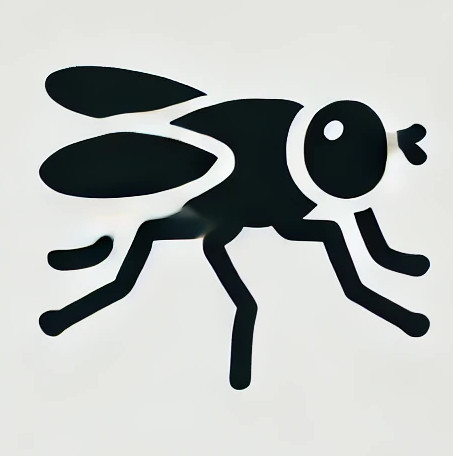
\includegraphics[width=2cm]{images/mucha.jpg}};
                \node [left= 0.5cm of A]{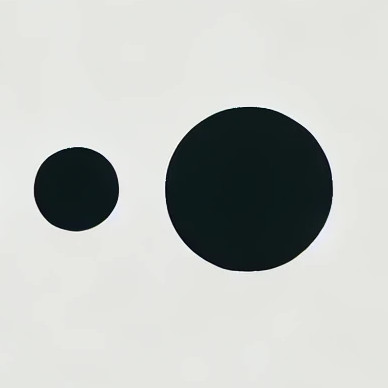
\includegraphics[width=2cm]{images/kropki.jpg}};
                \node [right= 0.5cm of Y]{
\includegraphics[width=3cm]{images/zaba.jpg}};
            
                % Titles
            
                
                % Arrows and connections
                \draw[thick,->] (A) -- (Y); % Arrow from left circle to ellipse
                \draw[->, thick] (B) -- (Y); % Arrow from diamond to ellipse
                
            \end{tikzpicture}
           
            

    \end{frame}


\begin{frame} 
    \begin{center}
      {\Huge  Kinds of information and their vehicles } % Use \Huge for very large font size
    \end{center}
\end{frame}






\begin{frame}{Semantic information and its vehicles}
 
We know well many examples of vehicles of semantic information:
 
Obvious cases:
\begin{itemize}
    \item true sentences (e.g. "The cat is on the mat" refering to the state of the world)
    \item maps of domains (e.g. terrain).
    \item photos and pictures, paintings.
\end{itemize}

Controvertial cases:
\begin{itemize}
    \item false sentences
    \item distorted images
    \item empty descriptions (e.g. "the king of France")
   
\end{itemize}

\textbf{\color{red} Three important comments here:}
\begin{itemize}
    \item All these cases "derive" or "inherit" their semantic information from mental content ("non-natural information"). 
   \item For sake of simplicity, I will equate them with structural representations (below)
    \item They are not only structural, but in most cases compositional.
\end{itemize}

 \end{frame}


 \begin{frame}{Conditions on structural representaions and its vehicles}

    Structural representations should meet the job description (\cite{ramsey_representation_2007}) for representations (\cite{gladziejewski_explaining_2015-1,gladziejewski_structural_2017}). 
 
     \begin{itemize}
         \item \textbf{Structural Similarity Condition:} The component part of the mechanism (the representational vehicle) should have a structural resemblance to the object it represents. 
         Important: misrepresetation is always  possible, because similarity comes in degrees.
         
         \item \textbf{Action-Guidance Condition:} The representation must guide the actions of the larger cognitive system.
         
         \item \textbf{Decouplability Condition:} The representation should be able to function even when the object it represents is not present.
         
         \item \textbf{Error-Detection Condition:} The system using the representation must have the ability to detect when the representation is inaccurate or false. 
     \end{itemize}

 
 \end{frame}



\begin{frame}{Similarity can be well defined }
    
    \begin{itemize}
        \item Similarity is a crucial aspect of representation, ensuring that the essential relationships and properties of the represented domain are maintained in the representing domain. 
        
        \item Similarity can be defined with the concept of homomorphism, which is a mapping that preserves the structure of set of objects and its map. Another way is defining similarity by abstract distance between some objects (e.g. strings "000000" and "00010" are quite similar, but not equal). This kind of similarity can be measured and is very natural in Shannon's theory toolkit.
       
        \item In the context of representation, homomorphisms ensure that the representing domain accurately reflects the structure of the represented domain, allowing for  inferences and predictions. 
    
  
    \end{itemize}
    
\end{frame}


\begin{frame}{Shannon information and its vehicles}

   The interesting cases of the vehicles of Shannon information are:
    \begin{itemize}
       
        \item binary strings (e.g. sequences of bits)
        \item words (e.g. in a newspaper)
        \item DNA sequences 
        \item waggle dance of honeybees
        \item neural spike trains (or some other aspects of bioelectric activity of neurons)
       
        \item ..any collections of any objects have information-theory properties such as entropy,and mutual information with some (other) collection. 
        
        
    \end{itemize}

\end{frame}


\begin{frame} { Shannon information and its vehicles (a very short intro) }
   
   Since Hartley (\cite{hartley_transmission_1928})  we can think about information as a non-psychological, quantifiable aspect of groups of objects, that could be carried or stored or transmitted or processed whatever these objects are. 

Shannon  extended Hartley’s approach, and introduced a statistical concept of entropy to measure this property. To compute the entropy of  the collection, we need only to know the distribution of it, that is the probabilities of elements in the collection.



\end{frame}


\begin{frame} { Shannon informtion and its vehicles (a very short intro) cont. }
The entropy of $X$ is defined as:
$$
H(X) = -\sum_{x \in \mathcal{X}} p(x) \log_2 p(x)
$$

where:
\begin{itemize}
    \item $H(X)$ is the entropy of the random variable $X$.
    \item $\mathcal{X}$ is the set of all possible values of $X$.
    \item $x$ is a specific value of $X$.
    \item $p(x)$ is the probability of $X$ taking the value $x$.
\end{itemize}

\textbf{"It measures the variability of the elements within a given distribution, giving it a crisp intuitive meaning that is general and applicable to all branches of science"} \cite{carcassi_variability_2021} 

The amount of Shannon information is then a statistical property of its vehicles. 
  
\end{frame}



\begin{frame}
    \begin{center}
      {\Huge 2. The Gap. Why suspect there is  more than one kind of information?} % Use \Huge for very large font size
    \end{center}

    \bigskip
    
    There is an abundance of arguments for the existence of more than one kind of information, here I will recall three of them.


\end{frame}

\begin{frame} {Levels of Organisation / Leibniz's mill argument} 
   
    \begin{itemize}
    
        
      \item  Rathkopf calls this state of affairs a bifurcation: "At a high level of neural organization, brain information is semantic, but down at the level of single neurons, semantic properties are irrelevant, and the only information to speak of is Shannon information."  (\cite{rathkopf_what_2020})
      
     
    \end{itemize}
      
  
  \end{frame}

\begin{frame}{Dennett's Trafalgar Square Argument}
    
    Dennett provides a toy model to illustrate the gap (\cite{dennett_bacteria_2017}): 
    
    "Jacques shoots his uncle dead in Trafalgar Square and is apprehended on the spot by Sherlock. Tom reads about it in the Guardian, and Boris learns of it in Pravda.\textbf{ Jacques, Sherlock, Tom, and Boris have had remarkably different experiences, but they share one thing: semantic information that a Frenchman has committed a murder in Trafalgar Square.} (...) They share no encoding, but they do share semantic information."

    \bigskip
    
    \begin{quote}
    "Semantic information, the concept of information that we must start with, is remarkably independent of encodings, in the following sense: two or more observers can acquire the same semantic information from encounters that share no channel" ()\cite{dennett_bacteria_2017}). 
    \end{quote}

    I will argue below that "seeing" these channels is a ambitious, open scientific project.

\end{frame}






\begin{frame}{Argument from Equal Entropy}
  Two different distributions can have the same Shannon entropy, $H(X)$, even if their internal structures differ significantly. 

\begin{center}
    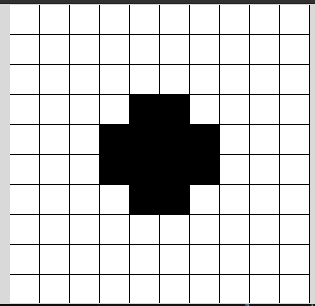
\includegraphics[width=0.25\textwidth]{images/entropia_1.png}
    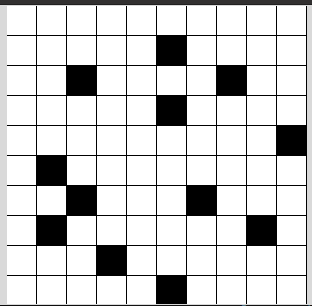
\includegraphics[width=0.25\textwidth]{images/entropia_2.png}
\end{center}
   The first receptive field may represent tasty food that some  fish could eat. Second is rather only a dirt! So the information first differs from the information in second one.
\end{frame}

\begin{frame}{Argument from Equal Entropy (cont.)}    
       
This argument is flawed in at least two respects.

First, whats is equal, is only the measure (entropy). Cf. a glass of water can carry the same amout of water as a bottle.    Shannon entropy captures the variability or uncertainty of a distribution but \textbf{does not capture the specific arrangement or structure of the data}.


    So the collorary is mistaken: it is not the case that there is a new kind of information, but rather that we should look for mechanism preserving order  or internal structure.

    E.g. in retina this order may be preserved just by spatial encoding that is then encoded by time relations between spikes

   


\end{frame}




\begin{frame}{The core of information theory}
Shannon information theory is more than Dretske  first used when starting his program of naturalizing knowledge.  
    \textbf{Crucially, it posits a mechanism called famously "Shannon communication model".}  This model has a task function.

“The fundamental problem of communication is that of reproducing
at one point either exactly or approximately a message selected at
another point.” (\cite{shannon_mathematical_1948})
\textbf{
Shannon model's task function, we mights say, is  optimizing reliabilty of transfer. What ELSE it is able to perform, is an open question}
    
Information theory has the communication model in its ontological commitments. When applied, the model equates to a kind of mechanism or is a part of bigger mechanism (in the sense of New Mechanists, \cite{machamer_thinking_2000,glennan_rethinking_2002}).
    
    Probably the best way to think about this mechanism is in terms of "information processing pipeline" (\cite{martinez_representations_2019}).
    Two of its 5 parts (encoder and decoder) are allowed to process information in any way that improves reliability of transmission of information.

    Importantly, this is a abstract mechanism description that we can map on many biological phenomena, organs, parts of organisms etc. But this practce is problematic (Nizami \cite{nizami_information_2019}).

    3 main theorems in the core of the information theory  relate to  different parts of the model: these are source coding theorem, channel coding theorem, and rate distortion theorem. They describe COMPRESSION  RATE LIMITs (resp. lossless transmission, lossy compression, and trade off between rate and distortion) of the communication model.


\end{frame}





\begin{frame}{ Shannon Model (\cite{shannon_mathematical_1948})}

    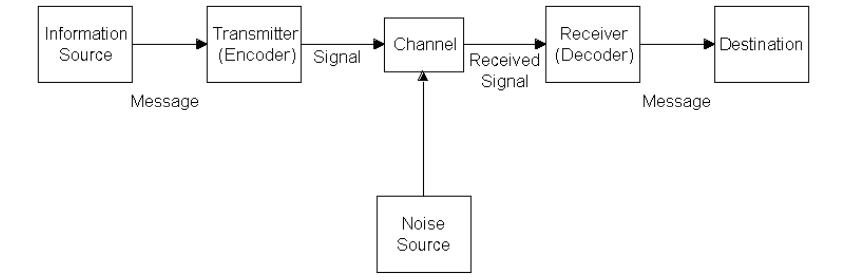
\includegraphics[width=1\linewidth]{images/latexImage_9d58f9e54772e4e91104b2b791c5c63e.png}
    
    \begin{tikzpicture}[remember picture, overlay]
        % Example: Placing a text node at a specific position over the imagethey
        \node at (1.5cm, 3cm) {\huge \textbf{\textcolor{red}{X} }};
        \node at (12.5cm, 3cm) {\huge \textbf{\textcolor{red}{$\hat{X}$}}};
        \node at (5cm, 3cm) {\huge \textbf{\textcolor{red}{encoder}}};
         \node at (9cm, 3cm) {\huge \textbf{\textcolor{red}{decoder}}};
    \end{tikzpicture}


Encoder and decoder are  machines performing some algorithms  in the given implementation.
The elements of the pipeline are then in \textbf{causal relations.} ("Cheap correlations" allegations can be then dismissed, if we are sure about the causal relations between the elements of the pipeline - if they are established independently)

    The whole pipepeline is also a machine, a stochastic one, when a channel is noisy.
    {$\hat{X}$} predicts or guesses the value of $X$.
   

\end{frame}


\begin{frame}{Shannon model as mechanism}
 
    The classic Shannon channel is a mechanism in this sense.
    According to the New Mechanists:

    Mechanisms are entities and activities organized in such a way that they are
    productive of regular changes from start or set-up to finish or termination conditions.
    (...)
    Mechanisms are composed of both entities (with their properties) and
    activities. Activities are the producers of change. Entities are the things
    that engage in activities. (\cite{machamer_thinking_2000})

    
    "A mechanism underpinning a behavior is a complex system that produces
    that behavior by the interaction of a number of parts, where the
    interactions between parts can be characterized by direct, invariant,
    change-relating generalizations." (\cite{glennan_rethinking_2002})

   

\end{frame}



\begin{frame}{ Semantic properties of Shannon pipeline }

        \begin{figure}[h!]
            \centering
            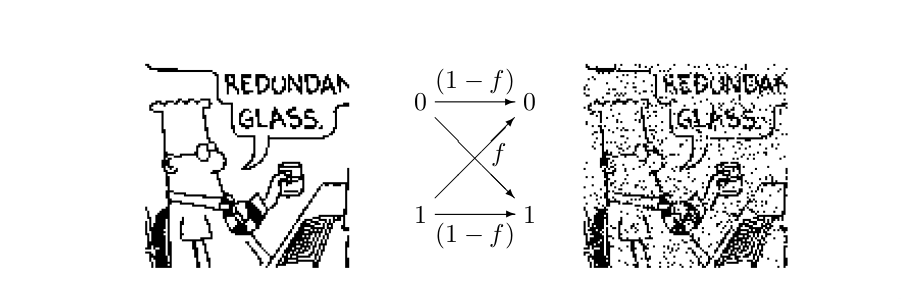
\includegraphics[width=1\linewidth]{images/Dilbert.png}
            \caption{Image transmitted through noisy channel, probability of bit flip = $f$ (\cite{MacKay2003})}
        \end{figure}
    
        \begin{tikzpicture}[remember picture, overlay]     
            \node at (4cm, 6cm) {\textbf{\textcolor{red}{accuracy condition}}};
             \node at (11cm, 6cm) {\textbf{\textcolor{red}{ semantic information}}};
        \end{tikzpicture}

        Accuracy conndition is the Source in the pipeline.
        Shannon model, when applied to cognitive subsystem of an organism, has accuracy conditions; that accuracy can be measured by mutual information between the source and the destination. Thus, the pipepile  is semantic: it is grounded in the Harnad sense (\cite{harnad_symbol_1990})

\end{frame}



\begin{frame}
    \begin{center}
      \Huge A candidate for structural representation
    \end{center}
\end{frame}






\begin{frame}{Why Shannon model is a good candidate for a structural representaton?}
    \begin{itemize}
        \item \textbf{Structural Similarity Condition - } The Shannon model inherently preserves the {\color{red} probabilistic structure} of the source and the transmitted signal, ensuring a degree of resemblance between the input and output.
        \item \textbf{Action-Guidance Condition - } The encoded and transmitted information carried by parts-vehicles of the model can guide actions in systems that  utilize the signal, such as neural networks.
        \item \textbf{Decouplability Condition -} The Shannon model allows for the transmission or storage of information independently of the presence of  source, enabling decoupled representations (hallucinations are possible and can be common). 
        \item \textbf{Error-Detection Condition -} The original Shannon model implements mechanism for error correction by design.
    \end{itemize}

    {\color{red}  Notice: probabilistic structure is not the same as rigid structure in the sense of compositionality. This is I thnik  one of the reasons for imperfect inferetial capabilities of large language models. }
    
\end{frame}




\begin{frame}{Why Shannon model is a good candidate for structural representation (cont.)?}
    \begin{itemize}
        
        \item Compression  algorithms can be used to reduce the amount of information transmitted while preserving the essential structure of the data. (information processing efficiency implies less energy spending)
        
        \bigskip
\textbf{        {\color{red} Below I claim more }
}     
        \item \textbf{Compositionality.} The model can be extended to handle \textbf{noisy addition}, allowing for the representation of complex structures and relationships, which is essential for compositionality of representations.
       
       \textbf{ This condition, I think, closes the gap between semantic information and Shannon informationl}
    \end{itemize}

   
\end{frame}



\begin{frame}{ Probabilistic Assumptions of Shannon Model \\ (\cite{shannon_mathematical_1948})}

    Multiple use of channel is assumed with no relation between elements of the sequence transmitted (for generality of Shannon theorems). Real world sources produce ordered signals.

\textbf{    1. Properties of source sequences : indendence of elements in sequence  }

$$
A_1, A_2, \ldots A_k \rightarrow \Gamma \rightarrow B_1, B_2, \ldots B_k
$$
independence of symbols:
$$
p\left(b_1, b_2, \ldots b_k \mid a_1, a_2 \ldots a_k\right)=p\left(b_1 \mid a_1\right) \cdot p\left(b_2 \mid a_2\right) \cdot \ldots \cdot p\left(b_k \mid a_k\right)
$$
no memory:
$$
p\left(b_k \mid a_1 \ldots a_k, b_1 \ldots b_{k-1}\right)=p\left(b_k \mid a_k\right)
$$
no feedback:
$$
p\left(a_k \mid a_1 \ldots a_{k-1}, b_1 \ldots b_{k-1}\right)=p\left(a_k \mid a_1 \ldots a_{k-1}\right)
$$


(Niwiński, lectures)

\end{frame}



\begin{frame} {Why order is  preserved on this conditions in the transmission at all?}

    This is simply a consequence of the construction of the channel!

    Shannon model processes the elements of sequences \textbf{"first in, first out"}, thus saving their order.

    So, if some order can be transferred, can there be homomorphisms achived?     And if we have hoomorphisms, we can have compositionality?

\end{frame}

\begin{frame}{ Shannon model with redundancy encoding and majority vote decoder}
    \textbf{   (Noisy) channel is defined as a matrix of conditional probabilities. }
    

    \begin{figure}[h!]
        \centering
        \begin{minipage}{0.6\textwidth}
            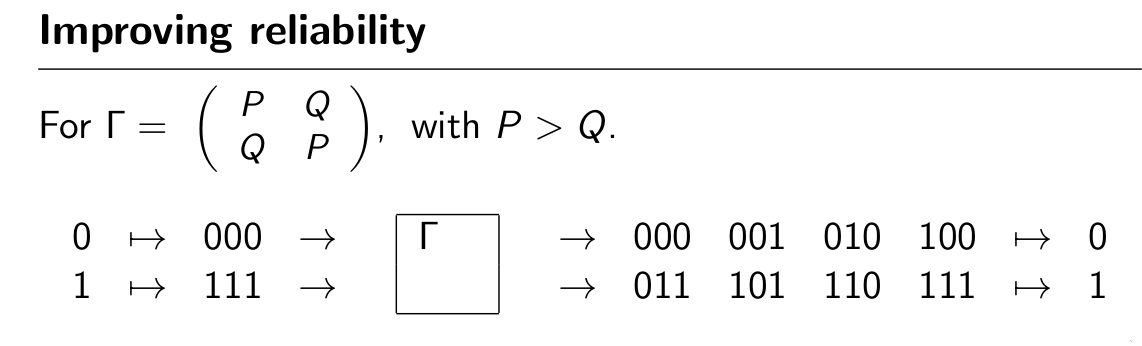
\includegraphics[width=\linewidth]{images/majority_vote.png}
            \caption{Majority vote rule}
        \end{minipage}
        \hfill
        \begin{minipage}{0.6\textwidth}
            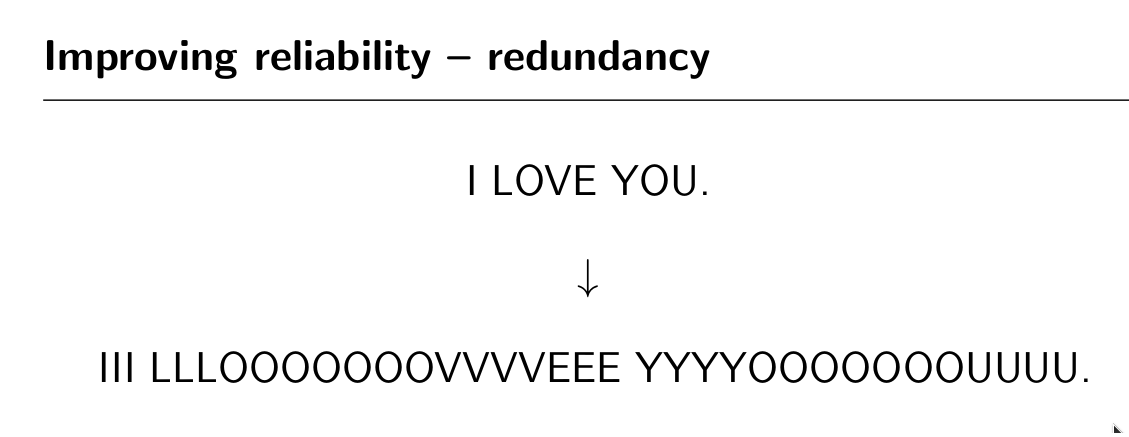
\includegraphics[width=\linewidth]{images/improving.png}
            \caption{Reliability improving mechanisms}
        \end{minipage}
     
    \end{figure}
    
    (Niwiński, lectures)
    
    \end{frame}









  

    \begin{frame} {It is not an easy task to see the Shannon channel}
    
        Now we may go back to Dennets argument for a while. Good mechanistic explanations should be able to map the elements of Shannon model on the cognitive pipelines. 
     
     The 3M requirement (\cite{kaplan_explanatory_2011-1} ) holds that for a model to count as a proper mechanistic explanation (as opposed to just a phenomenological description), it must satisfy two core conditions:
     
     The variables in the model must correspond to identifiable components, activities, and organizational features of the actual mechanism that produces, maintains, or underlies the phenomenon.
     
     The dependencies or relations posited among these variables in the model must correspond to causal relations among the components of the target mechanism
     
     But there is no consensus in neuroscience how to map them!   Cf.  Nizami's critique and his table from hell \cite{nizami_information_2019}
     He estimates the number of possible mappings of the Shannon model on the organisms for thousands. 
     
     
     \end{frame}

\begin{frame}  {But how to map Shannon Model? Nizami's table} 
   
  Nizami provides a table of possible mappings of the Shannon model onto the environment and parts of organisms. He estimates the number of possible mappings found in the literature for milions of possibilities. This is an open scientific project.
        \begin{center}
            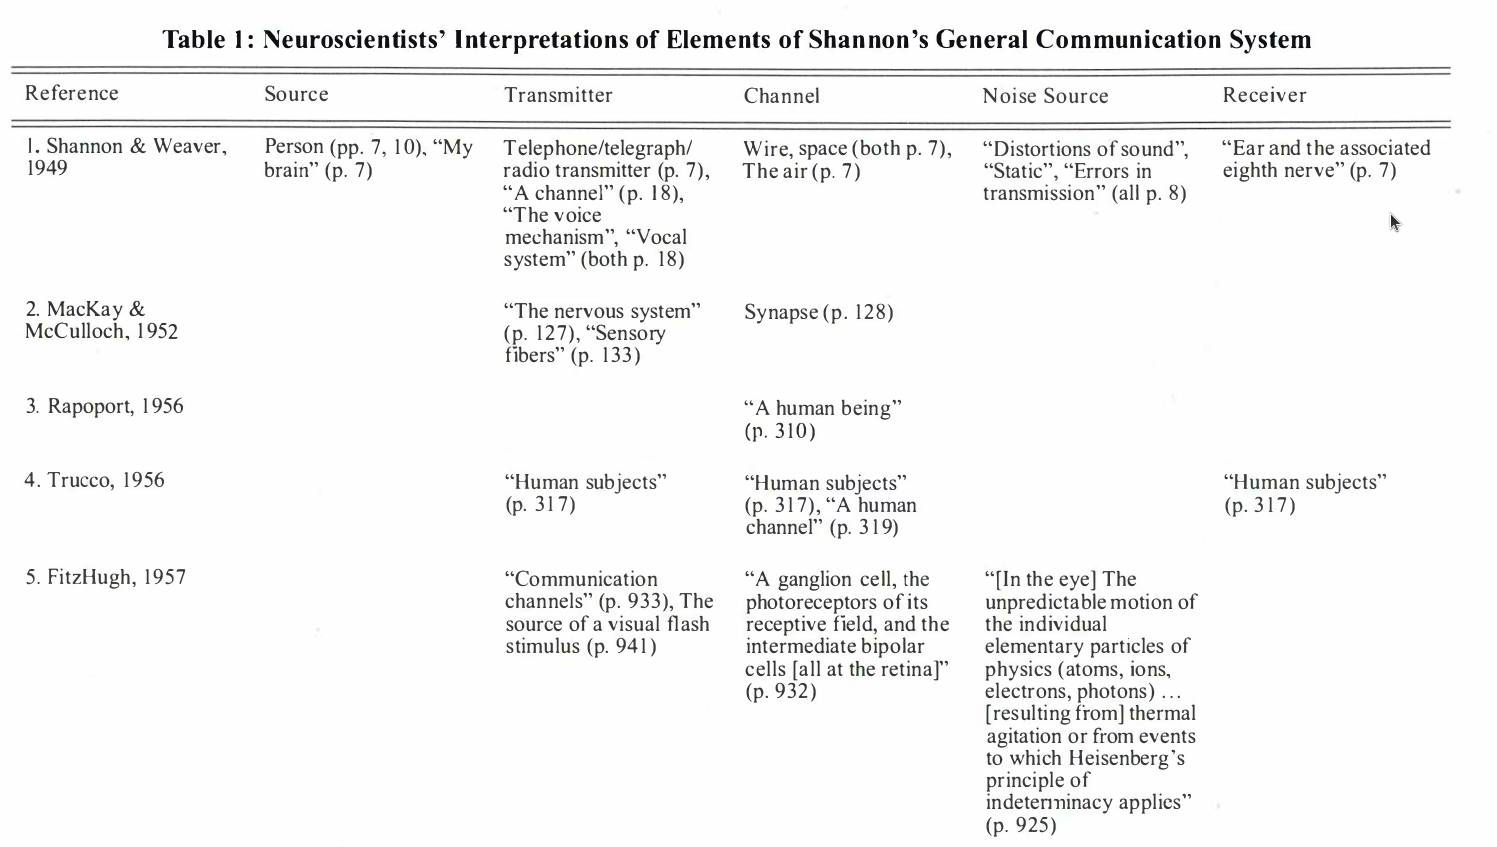
\includegraphics[width=1\textwidth]{images/Nizami_table1.png}
            \captionof{figure}{First page of Nizami's table of  mappings of the Shannon model in neuroscientific literature (\cite{nizami_information_2019}).}
        \end{center}

\end{frame}

\begin{frame}  {But how to map Shannon Model? Nizami's table cont.} 
    \begin{center}
        
       
            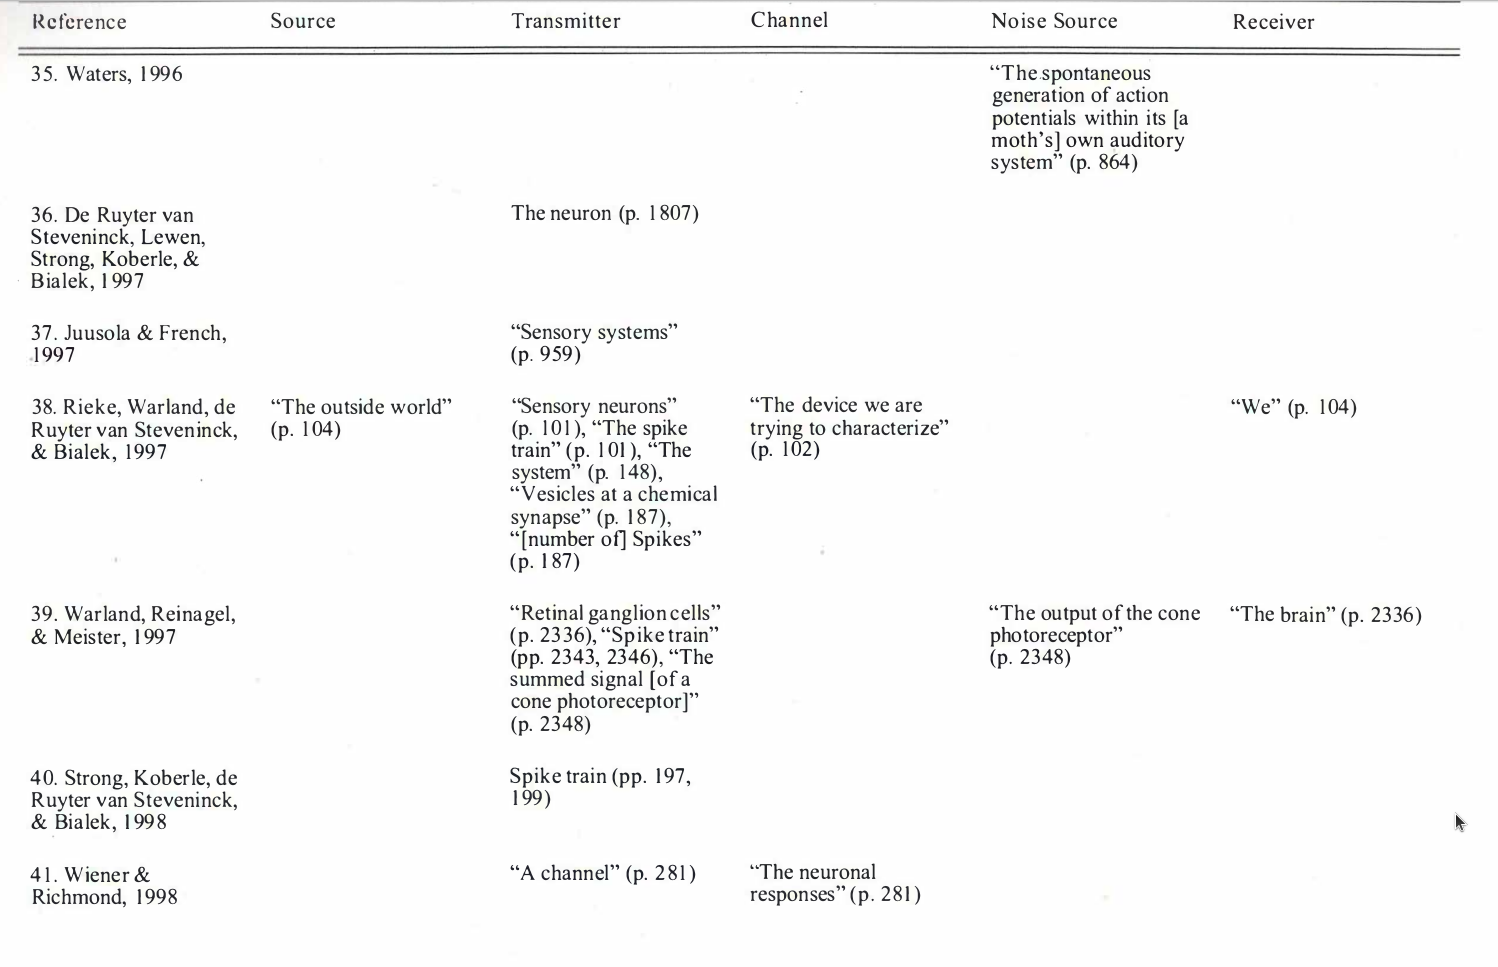
\includegraphics[width=1\textwidth]{images/Nizami_table2.png}
            \captionof{figure}{Last page of Nizami's table of  mappings of the Shannon model in neuroscientific literature (\cite{nizami_information_2019}).}
      


    \end{center}
\end{frame}







\begin{frame}{Phototaxis representational mechanisms: \\ semantic but not compositional}
    \small
    Something more sophisticated than thermostats: phototaxis (in algae) occurs when whole organisms move toward a light source for photosynthesis.
    
    \begin{columns}
        \begin{column}{0.5\textwidth}
            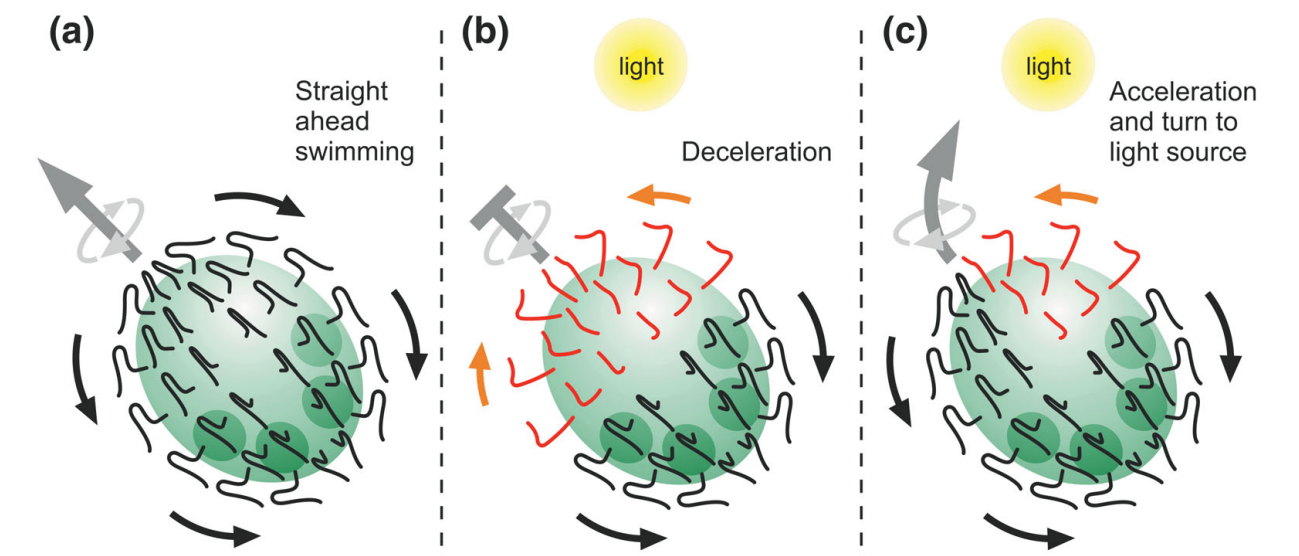
\includegraphics[width=\linewidth]{images/phototaxis.png}
        \end{column}
        \begin{column}{0.5\textwidth}
            \textbf{Phototactic movements in \textit{V. rousseletii}:}
            \begin{itemize}
                \item  Straight-ahead swimming in the dark.
                \item  A sudden dark-light switch reverses flagellar beating in the anterior hemisphere, decelerating forward motion (photophobic response).
                \item  After 2 seconds, only the illuminated side's cells reverse flagellar beating, turning the spheroid toward the light.
            \end{itemize}
            \tiny \textit{Adapted from \cite{ueki_how_2010}}
        \end{column}
    \end{columns}
    
    \vspace{1em}
    
    We can measure mutual information between the "movement alphabet" \{\textit{stop, follow}\} and "receptive field" \{\textit{dark, dark-light, light-2s}\}. But this yields only a black-box type of IT-based explanation—the underlying encoder/decoder mechanisms remain unknown.\\
    
    This kind of phototaxis is not (even) a neurological mechanism.
    
    \end{frame}
    





\begin{frame}{Many forms of compositionality}

Somewhat paradoxically, most natural domain for compositionality are artificial laaguages (after Frege). Natural language includes many counterexamples (e.g. "red herring")

\begin{quote}
The meaning of a compound expression is a function of the meaning of its parts and of the syntactic rule by which they are combined (\cite{janssen_compositionality_2012,janssen_frege_2001})
\end{quote} 
Compositionality is a general property of \textbf{complex} representational systems, but not only languages:

It is essential for linear algebra on multidimensional spaces:
\begin{itemize}
   
    \item \textbf{Distributivity of scalar multiplication with respect to vector addition:} For all scalars $c$ and all vectors $u$ and $v$ in $V$, $c(u + v) = cu + cv$.
    \item \textbf{Distributivity of scalar multiplication with respect to scalar addition:} For all scalars $c$ and $d$ and all vectors $v$ in $V$, $(c + d)v = cv + dv$.
\end{itemize} (\cite{axler_linear_2024})


We can also think of source sequences this way: we model world with linear algebra in science.
\textbf{\color{red} But that is not what Shannon model supports out of the box: it does not provide arithmetical operations on real numbers.}


\end{frame}



\begin{frame}{Many forms of compositionality}
   

\begin{table}[h!]
\centering
\small % Reduce font size
\begin{tabular}{|p{2cm}|p{4cm}|p{3cm}|p{3cm}|}
\hline
\textbf{Property} & \textbf{Definition \& Core Idea} & \textbf{Mathematical/Structural Formulation} & \textbf{Example Contexts} \\ \hline
Linearity in Algebra & A system is linear if it satisfies additivity and homogeneity: the output for a sum or scaled input equals the sum or scaled output (superposition principle). & $f(x + y) = f(x) + f(y)$, $f(\alpha x) = \alpha f(x)$ & Linear maps, vector spaces, circuits \\ \hline
Compositionality in Language & The meaning of a complex expression is determined by its structure and the meanings of its parts. & --- & Syntax, semantics, formal languages \\ \hline
Homomorphism & A structure-preserving map between two algebraic structures of the same type, preserving operations and relations. & $f(x \cdot y) = f(x) \cdot f(y)$ (for operation $\cdot$) & Groups, rings, vector spaces \\ \hline
\end{tabular}
\caption{Comparison of Properties in Algebra and Language}
\label{tab:properties}
\end{table}


    
\end{frame}


\begin{frame}{Compositionality "from" vector spaces - Smolensky}

    Once system can perform linear operations in multidementional spaces,system can reconstruct recursive syntax (\cite{smolensky_tensor_1990})
\small
    \begin{tabular}{|c|c|c|c|c|}
    \hline {\begin{tabular}{l} 
    Structuring \\
    operation
    \end{tabular}} & \multicolumn{2}{|l|}{ Symbolic formalization } & \multicolumn{2}{|l|}{ Vector embedding formalization } \\
    \hline & Structures & Example & Example & Vector operation \\
    \hline Combining & Sets & $\left\{\mathrm{c}_1, \mathrm{c}_2\right\}$ & $\mathbf{c}_1+\mathbf{c}_2$ & Vector sum + \\
    \hline \begin{tabular}{l} 
    Role/filler \\
    binding
    \end{tabular} & Strings, frames & $A B=\left\{r_1: A, r_2: B\right\}$ & $\mathbf{r}_1 \otimes \mathrm{~A}+\mathbf{r}_2 \otimes \mathrm{~B}$ & Tensor product $\otimes$ \\
    \hline \begin{tabular}{l} 
    Recursive \\
    embedding
    \end{tabular} & Tree & & \begin{tabular}{l}
    $\mathbf{r}_0 \otimes \mathrm{~A}$ \\
    + \\
    $\mathbf{r}_1 \otimes\left[\mathbf{r}_0 \otimes \mathbf{B}+\mathbf{r}_1 \otimes \mathbf{C}\right]$
    \end{tabular} & \begin{tabular}{l} 
    Recursive role \\
    embeddings: \\
    $\mathbf{r}_{\text {child }_{0 / 1}}(x)=\mathbf{r}_x \otimes \mathbf{r}_{0 / 1}$
    \end{tabular} \\
    \hline
    \end{tabular}
    
    Combinatorial neural representations: Tensor Product Representations 
    - The vector embedding the whole is the sum of the vectors embedding the constituent role/symbol bindings:
    $$
    a(\text { structure })=a\left(\mathrm{R}_1: \mathrm{S}_1\right)+a\left(\mathrm{R}_2: \mathrm{S}_2\right)+\cdots
    $$
   
    
    \end{frame}



\begin{frame}{S-representations seem to exist in convolutional neural networks}
\small
    \begin{columns}
        \begin{column}{0.5\textwidth}
            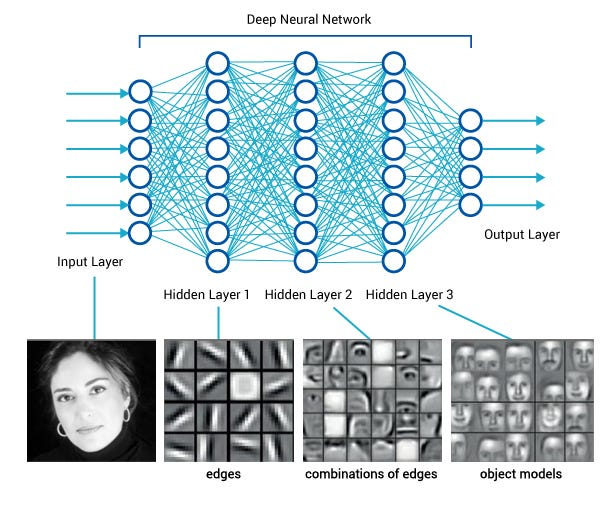
\includegraphics[width=\linewidth]{images/cnn.jpg}
        \end{column}
        \begin{column}{0.5\textwidth}
            Structural representations (and metarepresentations) seem to exist in CNNs.
    
            \begin{itemize}
                \item \textbf{\color{red}Structural similarity} to the features present in training data (but homomorphisms can be hard to identify). Are they compositional? Not fully or not at all (constant problems with inferences in large language models).
                \item \textbf{\color{red}Veridical}: classify with accuracy  open classes of examples (mis)representation capabilities.
                \item \textbf{\color{red}Contentful}: clusters of vectors in weight matrices can represent Dennet's "real patterns" or natural kinds.
            \end{itemize}
        \end{column}
    \end{columns}
    
    \vspace{0.5em}
    \textbf{Can we express a structural representation by pure means of information theory?}
  
    
    \end{frame}
    

\begin{frame}
    \frametitle{How (convolutional) artificial neural preserve structure?}
    \textbf{They use numbers.}
    The smallest building blocks of most of the  networks (artificial neurons) use  linear algebra and compute sums of weighted inputs, which is a linear, compositional  operation.    
    
    \textbf{To fit them in the Shannon model picture let us assume that the incoming elements of a sequence are ordered} - as in binary code.  The sequences of objects from the alphabet set \(\{0,1\}\) in the input signal are then ordered from the most important to the least important (or from the strongest to the weakest). In this binary sequence, the first bit is the most important or the strongest, and the last bit is the least important or the weakest, with the \((n-1)\)-th element being two times weaker than the \(n\)-th element. 

For example, the sequence:
\[
a_{1..4} = 1011
\]
encodes a signal of intensity:
\[
2^3 + 2^1 + 2^0 = 11.
\]
    

\end{frame}


\begin{frame}{Biological Plausibility: Barlow’s hypothesis}

    \begin{columns}[T] % The [T] option aligns the columns at the top
   
           % Column for the picture
           \begin{column}{0.5\textwidth}
               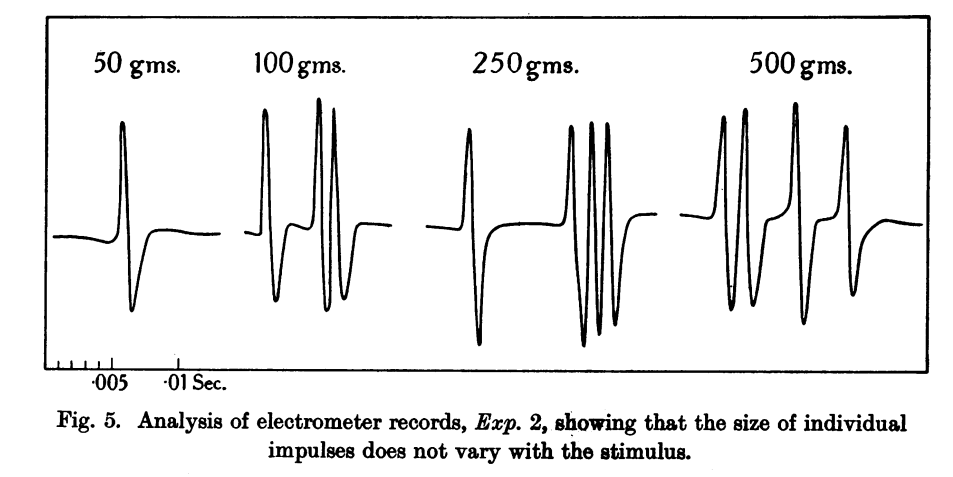
\includegraphics[width=1\linewidth]{images/latexImage_aad051c66a8ab8fe36b14843445faa7f.png} % Adjust the path and filename
           \end{column}
   
           % Column for the text
           \begin{column}{0.5\textwidth}
            Sensory neuron's firing rate reflects the strength of stimulation (Adrian, Zotterman, 1926), a higher rate indicating a stronger stimulation (but the size of each spike remains constant).
           \end{column}
   
       \end{columns}
   
   
   In 1953, Barlow hypothesized:

   \begin{itemize}
       \item \textbf{the stronger the stimuli, the richer are the spike trains} (interpreted as neuron's response to the stimuli).
   \end{itemize}
   
   Barlow hypothesized that the spikes in the sensory system formed a neural code for efficiently representing sensory information. \textbf{By efficient, Barlow meant that the code minimized the number of spikes needed to transmit a given signal.} 

\end{frame}



\begin{frame}{Main Question: How would adding be achievable in the Shannon model by means of information theory?}


    Notice that the McCulloch-Pitts  model already USES summation for its threshold logic (\cite{mcculloch_logical_1943})
   
     We know "some kind" of "sum" operation is performed by neurons.
     
     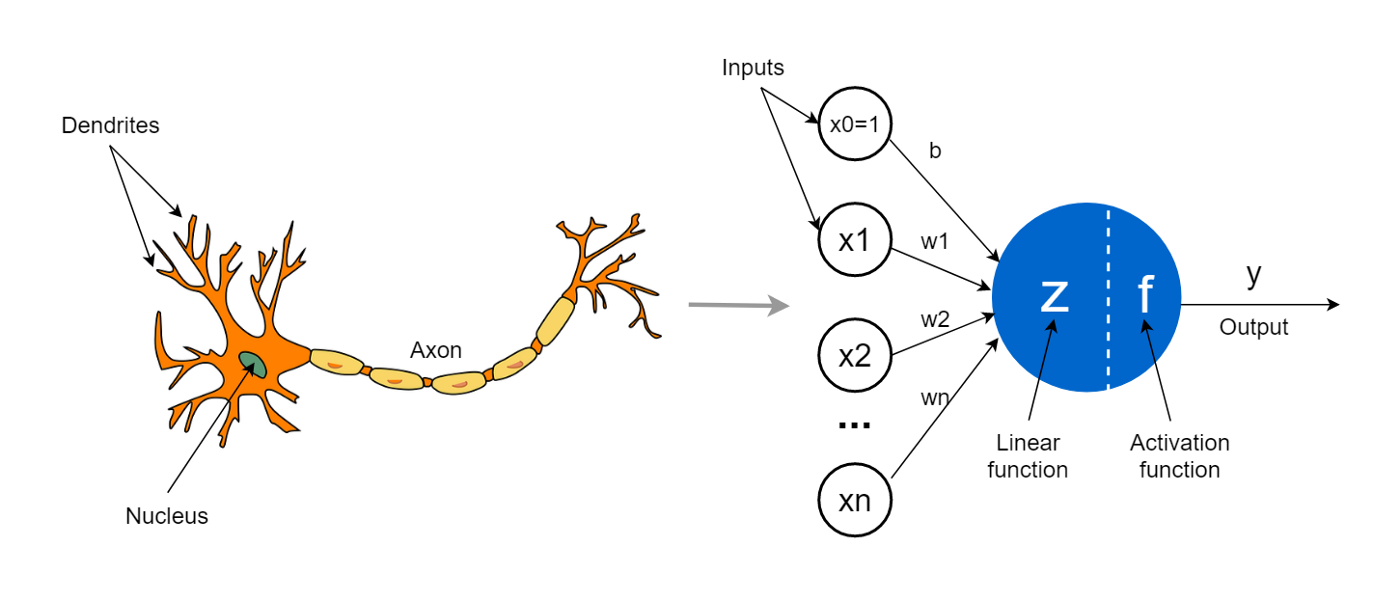
\includegraphics[width=10cm]{images/latexImage_63d4c13d6261c28a5b1ff9f3f41e4f0d.png}

  \textbf{ How is adding possible in the Shannon model by pure means of information theory?}
    
\end{frame}
 




\begin{frame}{Word2vec model: meanings as points (clusters) in multidimensional vector spaces}
    

    Distributional semantics: A word's meaning is given by the words that frequently appear close by (context)

    "You shall know a word by the company it keeps" (J. R. Firth 1957: 11)
    One of the most successful ideas in modern statistical NLP.
    When a word $w$ appears in a text, its context is the set of words that appear nearby (within a fixed-size window).

    Word2vec models (\cite{mikolov2013a}) are in fact weights of neural nets trained to recognize similar words as close vectors in multidimensional vector space.


\end{frame}

\begin{frame}{Traits of compositionality:  Mikolov effect and  analogies of predicates}

   Word models show that meaning (i.e linguistic representation) can be represented as points in multidimensional vector spaces, and whats more, complex meanings can be predicted from simple meanings by means of vector arithmetic (linear algebra)
    Consider the above approximation of meaning relation (\cite{mikolov2013a}):
   \huge $$\text{king} - \text{man} + \text{woman} \approx \text{queen}.$$

\end{frame}

\begin{frame}{Mikolov effect}

   
       
   \textbf{ Mikolov effect suggests that word embeddings space has linear and thus compositional properties}, as we can predict meaning of complex expressions from the meanings of their parts.
  

    What is the explanation of this effect?
    This effect is, I think,  due to  compositionality of meaning in vector spaces, where the meaning of a complex expression can be derived from the meanings of its parts and the way they are combined.
\textbf{
    But what is the scaffolding for this compositionality? How could it be achieved in the Shannon model? }
    
    I propose the construction that partly shows how linearity can be achieved in the Shannon model.

\end{frame}





\begin{frame}{Analogies between predicates: meaning prediction (since \cite{rumelhart_model_1973})}

    \begin{minipage}{0.45\textwidth}
    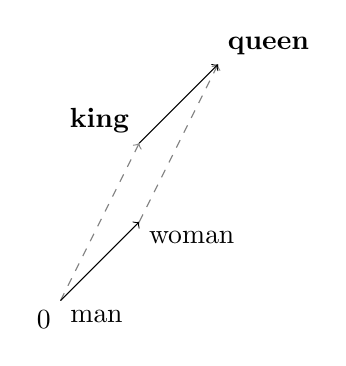
\begin{tikzpicture}
        % Points
        \coordinate (origin) at (0, 0);
        \coordinate (man) at (0, 0);
        \coordinate (woman) at (1, 1);
        \coordinate (king) at (1, 2);
        \coordinate (queen) at (2, 3);
    
        % Vectors
        \draw[dashed, gray, ->] (man) -- (king);
        \draw[dashed, gray, ->] (woman) -- (queen);
        \draw[black, ->] (man) -- (woman);
        \draw[black, ->] (king) -- (queen);
    
        % Points labels
        \node[below left] at (man) {0};
        \node[below right] at (woman) {woman};
        \node[above left] at (king) {\textbf{king}};
        \node[above right] at (queen) {\textbf{queen}};
        \node[below right] at (man) {man};
    
    \end{tikzpicture}
    \end{minipage}
    \hfill
    \begin{minipage}{0.45\textwidth}
    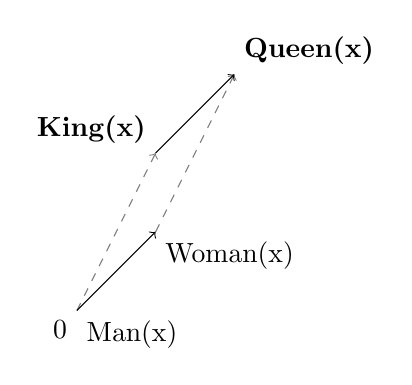
\begin{tikzpicture}
        % Points
        \coordinate (origin) at (0, 0);
        \coordinate (man) at (0, 0);
        \coordinate (woman) at (1, 1);
        \coordinate (king) at (1, 2);
        \coordinate (queen) at (2, 3);
    
        % Vectors
        \draw[dashed, gray, ->] (man) -- (king);
        \draw[dashed, gray, ->] (woman) -- (queen);
        \draw[black, ->] (man) -- (woman);
        \draw[black, ->] (king) -- (queen);
    
        % Points labels
        \node[below left] at (man) {0};
        \node[below right] at (woman) {Woman(x)};
        \node[above left] at (king) {\textbf{King(x)}};
        \node[above right] at (queen) {\textbf{Queen(x)}};
        \node[below right] at (man) {Man(x)};
    
    \end{tikzpicture}
    \end{minipage}
    
   
    
\end{frame}


\begin{frame}{A proposal for noisy addition model }
   
\textbf{How can computaional model acuire linear capabilities by exploting the Shannon model pipeline?}
    
Let me now propose that the "mutated" or "exapted" Shannon channel can perform computation: specifically, (noisy) addition without relying on traditional arithmetic operations. Why choose addition? 

Having addition, system could gain the task function of "measuring intensity," which leads to thresholding units (\cite{mcculloch_logical_1943}) and, consequently, to classification capabilities and linear properties in the system.

Consider two channels \(\Gamma_1\) and \(\Gamma_2\) present in an agent—say, a worm \(S\). Together, they transmit signals from the frontal part to the rear motor part of the worm. The signals are transmitted as binary sequences.


\[
S \underset{\text{code}}{\mapsto} A \rightarrow \boxed{\Gamma_1} \rightarrow B \underset{\text{decide}}{\mapsto} \Delta(B) \underset{\text{decode}}{\mapsto} S
\]

\[
S \underset{\text{code}}{\mapsto} A \rightarrow \boxed{\Gamma_2} \rightarrow B \underset{\text{decide}}{\mapsto} \Delta(B) \underset{\text{decode}}{\mapsto} S
\]

\end{frame}

\begin{frame}{A proposal for noisy addition model (cont.) }

\textbf{Now, suppose the channel \(\Gamma_2\) breaks—its receiver fails.} 

The exapted model is now represented as follows:

\[
S \underset{\text{code}}{\mapsto} A \rightarrow \boxed{\Gamma_1} \rightarrow B \underset{\text{decide}}{\mapsto} \Delta(B) \underset{\text{decode}}{\mapsto} S
\]

\[
S \underset{\text{code}}{\mapsto} 
A 

\begin{tikzpicture}[overlay, remember picture]
    \draw[->, red, thick] (0,0) to[out=90,in=200] (0.6,0.9);
\end{tikzpicture}
\textcolor{white}{\rightarrow }
\textcolor{lightgray}{\boxed{\Gamma_2} \rightarrow B \underset{\text{decide}}{\mapsto} \Delta(B) \underset{\text{decode}}{\mapsto} S}
\]

\textbf{Surprisingly, this pipeline is able to perform addition, with given noise. }

\end{frame}


    

\begin{frame}{A proposal for noisy addition model (cont.)}
   
    A plot of outputs of the proposed noisy adder. Depending on noise level it may add better or worse; its main advantage is biological plausability
        
        \begin{figure}[h!]
            \centering
            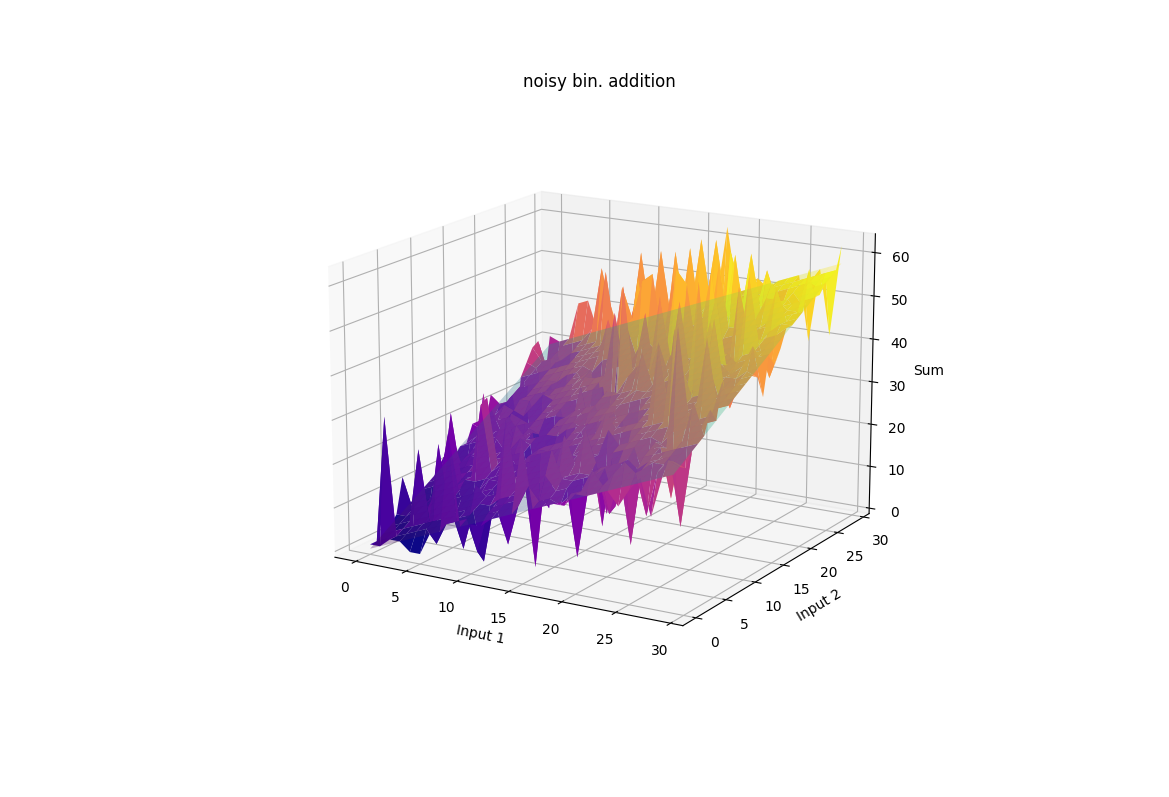
\includegraphics[width=0.7\textwidth]{images/anoisy_adding.png}
            \caption{}
            \label{fig:noisy_adder}
        \end{figure}
    
    
    
    \end{frame}
    


    
    \begin{frame}{Conclusions }
    
        \begin{itemize}
            To explain semantic phenomena is to provide a description of the pipeline that processes the variabilty (Carcassi),  what seems like proper scientific task with some prospect of successes.
          
            \item To explain  structural representations, only one kind of information is needed: "Shannon" information. When processed by complex pipelines (e.g., neural networks), it does not become  (1) semantic nor (2) compositional: the whole pipeline has this properties  and qualifies as an S-representation. Our ontology gets healtier. 
            
\textbf{    c.f. John does not become car-ish when driving a car.
}
            \item There is a mechanistic, biologically plausible transition from the original Shannon model to machine learning models such as classifiers (e.g. CNNs). I suggest the minimal improvemnt towards that kind of pipeline is the proposed here "noisy adder".
            
            \item Full, proper explanation of cognitive pipeline is a scientific project of finding the right model of the pipeline that processes the variability (Carcassi) and properly maps it's parts, following 3M rule (\cite{Craver}).
        \end{itemize}
      
    \end{frame}
    
    
    \begin{frame}
        \begin{figure}[h!]
            \centering
            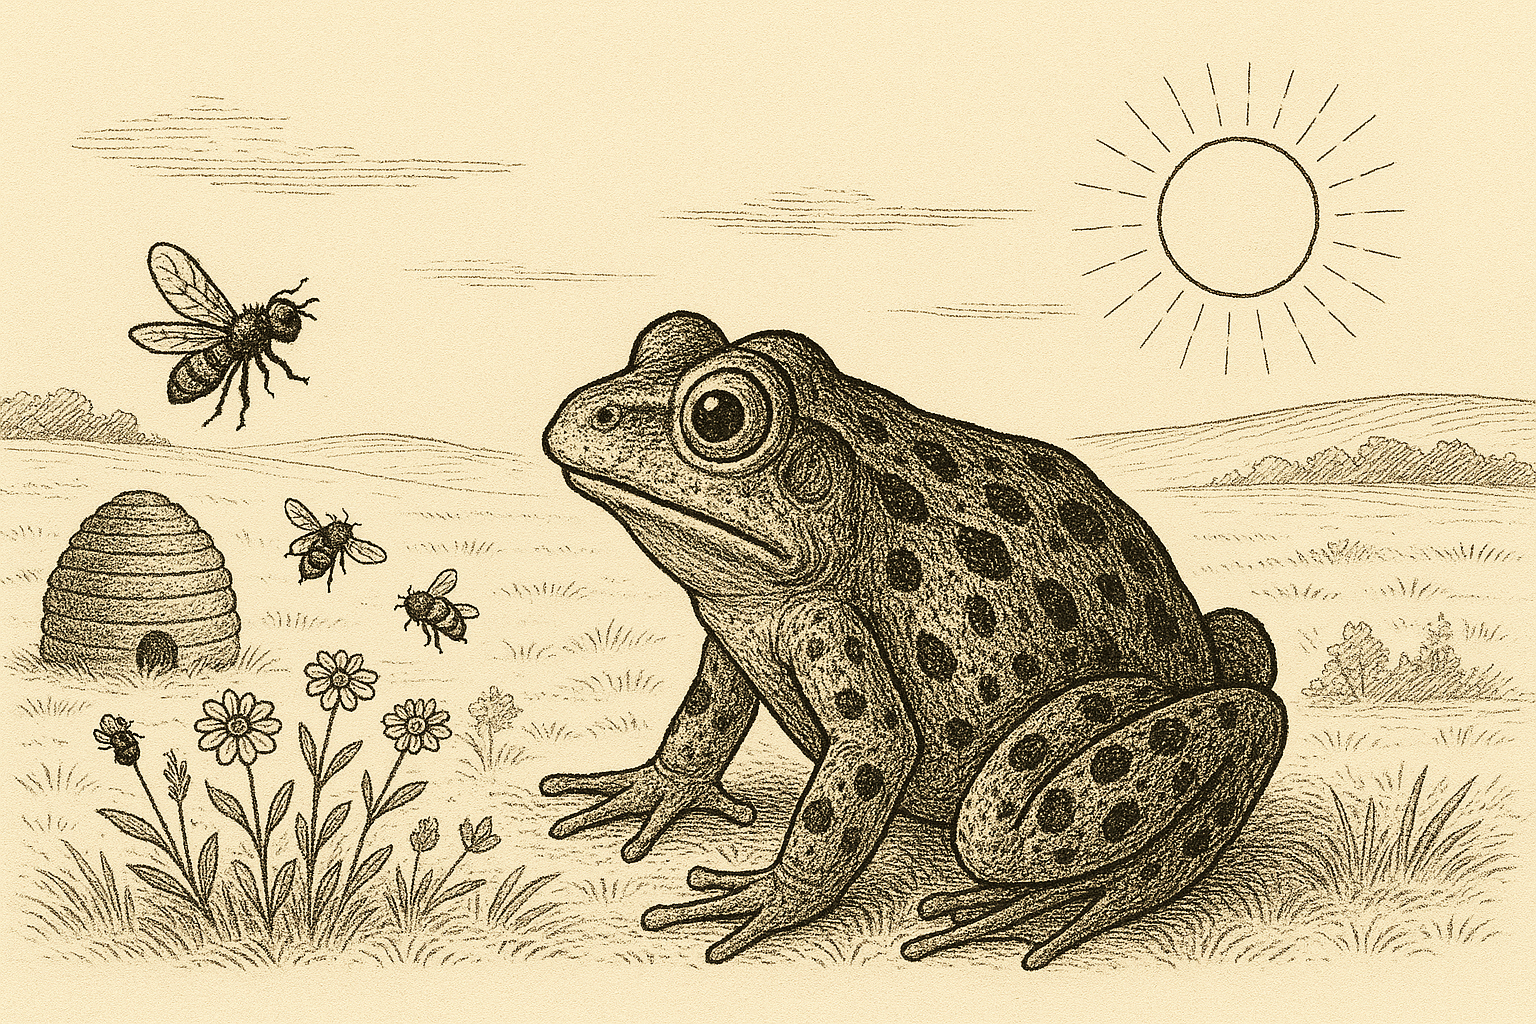
\includegraphics[width=0.8\textwidth]{images/frog_world.png}
            \caption{\Huge Thank you. Represent! }
            
        \end{figure}
      
    \end{frame}
    
    

    \begin{frame}[allowframebreaks]{References}
   \small
        \printbibliography
    \end{frame}



        \end{document}



% \begin{frame}{Bullets entering one at a time}
%     \begin{itemize}
%       \item Bullet 1
%       \onslide<2->{\item Bullet 2}
%       \onslide<3->{\item Bullet 3}
%       \onslide<4->{\item Bullet 4}
%     \end{itemize}
%   \end{frame}


